\pdfoutput=1
\documentclass[conference]{IEEEtran}
\IEEEoverridecommandlockouts

\usepackage{cite}
\usepackage{amsmath,amssymb,amsfonts}
\usepackage{algorithmic}
\usepackage{algorithm}
\usepackage{graphicx}
\usepackage{textcomp}
\usepackage{xcolor}
\usepackage{booktabs}
\usepackage{multirow}
\usepackage{url}
\usepackage{microtype}

\def\BibTeX{{\rm B\kern-.05em{\sc i\kern-.025em b}\kern-.08em
    T\kern-.1667em\lower.7ex\hbox{E}\kern-.125emX}}

\begin{document}

\title{RSA-SHIELD: Evidence-Correct RSA Public-Key Auditing with a Labeled Benchmark and Epistemic Tool Bake-Off}

\author{
\IEEEauthorblockN{Anonymous Author(s)}
\IEEEauthorblockA{\textit{Department and Affiliation Omitted for Double-Blind Review}\\
Paper Under Peer Review}
}

\maketitle

\begin{abstract}
RSA remains widely deployed in legacy industrial control, embedded devices, and enterprise PKI. Weak key generation can leave moduli factorable from public material alone, yet many scanners still treat a failed short probe as evidence that a key is ``secure.'' We present \textbf{RSA-SHIELD}, a defensive public-key auditor that \emph{never} emits an absolute \texttt{SECURE} label. We contribute: (i)~\textbf{RSA-Auditor Bench} with an epistemic bake-off; (ii)~a public CT tip sample; (iii)~\textbf{ROCA fingerprint parity} against \texttt{badkeys}; and (iv)~a \textbf{feature-adaptive probe scheduler} that preserves factor recall while cutting mean latency. On frozen dumps: bake-off overconfidence $0.0$ vs.\ \texttt{badkeys} $0.75$; legacy educational ROCA false-positive rate $75\%$ vs.\ \texttt{badkeys} on a CT tip sample ($n{=}500$), reduced to $0.2\%$ after threshold calibration (agreement $99.8\%$); adaptive scheduling achieves $1.511\times$ lower average wall time on Bench with recall still $1.0$. We do not claim a new factorization algorithm or a full Internet census.
\end{abstract}

\begin{IEEEkeywords}
RSA, public-key auditing, Certificate Transparency, evidence taxonomy, benchmark, batch GCD.
\end{IEEEkeywords}

\section{Introduction}
Since Rivest, Shamir, and Adleman introduced RSA~\cite{rivest1978method}, public-key systems have relied on the hardness of factoring $N{=}pq$. In practice, legacy SCADA/IIoT deployments and poorly seeded embedded generators produce moduli weak against public-key-only attacks~\cite{heninger2012mining,hastings2016weak,lenstra2012ron}: shared primes, near-twin primes (Fermat), small private exponents (Wiener)~\cite{wiener1990cryptanalysis}, Infineon-style ROCA structure~\cite{nemec2017return}, and small factors amenable to Lenstra ECM~\cite{lenstra1987factoring}.

\subsection{The Epistemic Flaw of Binary Labels}
Operational scanners often collapse cryptanalysis into pass/fail: if a short test returns no factor, the asset is marked ``PASS'' or ``SECURE.'' Cryptographically, \textit{failure to factor within a bounded budget is not a proof of security}. Offensive toolboxes such as \texttt{RsaCtfTool}~\cite{rsactftool} maximize CTF recovery but fit poorly in governed defensive audits. Passive scanners such as \texttt{badkeys}~\cite{bock2022badkeys} emphasize known-vulnerable fingerprints; empty findings are commonly read as ``OK,'' which is exactly the overconfidence failure mode we measure.

\subsection{Contributions}
\begin{itemize}
    \item \textbf{Evidence-tiered taxonomy + Bench/bake-off:} Never-\texttt{SECURE} labels; overconfidence vs.\ \texttt{badkeys} (Fig.~\ref{fig:bakeoff}).
    \item \textbf{ROCA parity + calibration:} Educational fingerprint vs.\ \texttt{badkeys}; calibrated thresholds cut CT tip FP $75\%\!\rightarrow\!0.2\%$ (Fig.~\ref{fig:roca}).
    \item \textbf{Adaptive probe scheduler:} Bit-length / exponent-driven budgets preserving recall at $1.511\times$ lower mean latency (Fig.~\ref{fig:adaptive}).
    \item \textbf{Multi-log CT sample + batch GCD:} $12010$ unique moduli from three public logs; Bernstein trees~\cite{bernstein2004find} (Figs.~\ref{fig:ct},~\ref{fig:batch}).
\end{itemize}
We do \emph{not} claim a novel general factorization algorithm, full CVE parity with \texttt{badkeys}/crocs-roca, shipped post-quantum CBOM generation, or a billion-certificate CT census.

\section{Threat Model and Audit Taxonomy}
RSA-SHIELD operates only on authorized public material (PEM/X.509 or raw $(N,e)$). Private exponents, primes, and ciphertexts are rejected at ingest. Probes are compute-bounded. Classification is epistemic:
\begin{enumerate}
    \item \textbf{\texttt{FACTOR\_FOUND}:} Non-trivial factor recovered (trial, Fermat, Wiener, ECM, or batch GCD).
    \item \textbf{\texttt{SUSPICIOUS}:} Heuristic warnings without a factor proof.
    \item \textbf{\texttt{INCONCLUSIVE}:} Active probes exhausted budget without a factor.
    \item \textbf{\texttt{NO\_WEAKNESS\_DETECTED}\ldots{}:} Configured checks passed; still not a security proof.
    \item \textbf{\texttt{INVALID\_KEY}:} Parse/parameter rejection.
\end{enumerate}

\section{System Architecture and Probing Pipeline}
\begin{figure}[t]
\centering
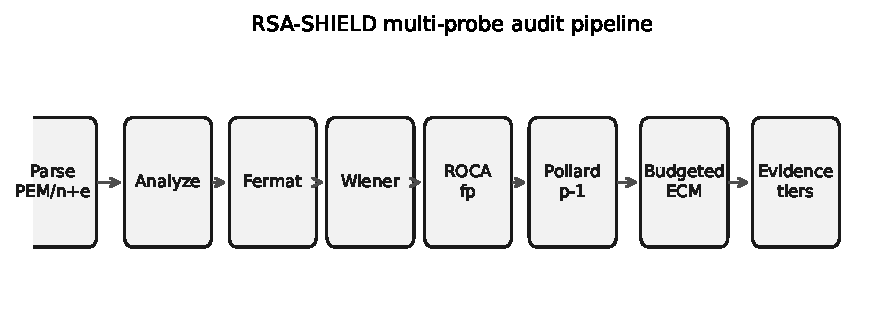
\includegraphics[width=\columnwidth,height=2.2in,keepaspectratio]{figures/fig_pipeline.pdf}
\caption{RSA-SHIELD audit pipeline. Factor recovery short-circuits later probes; failure to factor never yields \texttt{SECURE}.}
\label{fig:pipeline}
\end{figure}

FastAPI ingest, audit orchestration, algebraic probes, SQLite persistence, and a React evaluation UI implement Fig.~\ref{fig:pipeline} / Algorithm~\ref{alg:pipeline}.

\begin{algorithm}[t]
\caption{Budgeted multi-probe audit (orchestrator sketch)}
\label{alg:pipeline}
\begin{algorithmic}[1]
\REQUIRE Public key $(N,e)$; budgets $K_{\mathrm{Fermat}}$, $T_{\mathrm{ECM}}$
\ENSURE Evidence tier $\tau$; optional factor $p$
\STATE $\tau \leftarrow$ deterministic analyze$(N,e)$
\IF{factor found}
    \RETURN \texttt{FACTOR\_FOUND}, $p$
\ENDIF
\STATE Fermat ($\le K_{\mathrm{Fermat}}$); on hit \RETURN \texttt{FACTOR\_FOUND}
\STATE Wiener convergents of $e/N$; on hit \RETURN \texttt{FACTOR\_FOUND}
\STATE ROCA fingerprint may raise \texttt{SUSPICIOUS} (never a factor proof alone)
\STATE Pollard $p{-}1$ under B1/timeout; on hit \RETURN \texttt{FACTOR\_FOUND}
\STATE ECM under $T_{\mathrm{ECM}}$; on hit \RETURN \texttt{FACTOR\_FOUND}
\STATE Map warnings/timeouts to \texttt{SUSPICIOUS}/\texttt{INCONCLUSIVE}/configured-checks state
\STATE \textbf{assert} $\tau \neq$ \texttt{SECURE}
\RETURN $\tau$
\end{algorithmic}
\end{algorithm}

\subsection{Algebraic Probes}
\textbf{Fermat.} $N{=}a^{2}{-}b^{2}$ with call-site cap $K{=}25{,}000$ (library default $50{,}000$ overridden). Frozen \texttt{fermat-close} recovered a factor in $1$ step ($0.13$\,ms).
\textbf{Wiener.} Convergents of $e/N$ when $d{<}\tfrac13 N^{1/4}$~\cite{wiener1990cryptanalysis}; \texttt{wiener-small-d} recovered an approximately $45$-bit $d$ after $26$ convergents ($9.48$\,ms).
\textbf{ROCA fingerprint.} Educational residue/orbit heuristic~\cite{nemec2017return}; positive $\Rightarrow$ \texttt{SUSPICIOUS}, not Coppersmith factorization.
\textbf{Pollard's $p{-}1$.} Budgeted stage-1 smooth-order probe (B1-capped, wall-clock timeout) runs before ECM; recovers factors when some $p\mid N$ has $p{-}1$ smooth up to B1.
\textbf{Budgeted ECM.} Lenstra ECM~\cite{lenstra1987factoring} under timeout; ablation mean $1682.63$\,ms on weak fixtures.

\section{Subquadratic Batch-GCD Engine}
Shared primes are detectable by batch GCD~\cite{heninger2012mining}. RSA-SHIELD implements Bernstein product/remainder trees~\cite{bernstein2004find} with a pairwise baseline (Algorithm~\ref{alg:batch_gcd}).

\begin{algorithm}[t]
\caption{Subquadratic Batch-GCD (implementation sketch)}
\label{alg:batch_gcd}
\begin{algorithmic}[1]
\REQUIRE Moduli $\mathcal{M}=[m_0,\dots,m_{N-1}]$
\ENSURE Shared-factor hits $\mathcal{H}$
\STATE Build binary product tree $\mathcal{T}$ with leaves $\mathcal{M}$
\STATE Descend remainder tree: $R \leftarrow P \pmod{m^{2}}$ at each node
\FOR{$i=0$ \TO $N-1$}
    \STATE $g_i \leftarrow \gcd(m_i, \lfloor R_i / m_i \rfloor)$
\ENDFOR
\STATE Match pairs among indices with $1{<}g_i{<}m_i$; append hits to $\mathcal{H}$
\RETURN $\mathcal{H}$
\end{algorithmic}
\end{algorithm}

\section{Experimental Evaluation}
\label{sec:eval}
\subsection{Setup and Reproducibility}
Core suite/ablation/comparison/corpus/batch dumps were frozen by \texttt{paper/scripts/dump\_eval\_data.py} on 2026-11-13 (UTC \texttt{2026-11-13T08:55:11.449049+00:00}). CT tip, ROCA calibration/parity, and adaptive ablation dumps were frozen on 2026-11-18 on the same host. Host: Windows-10-10.0.26300-SP0, Python~3.11.9, ECM timeout $2500$\,ms, corpus size $40$, bench version $1.0.0$, \texttt{emits\_secure\_label}${=}$\texttt{false}. Artifacts: \texttt{paper/data/*.json}, \texttt{paper/benchmark/}, figures via \texttt{generate\_figures.py}. Milliseconds are machine wall-clock (no hand-edited cells).

\subsection{RSA-Auditor Bench}
Bench v1.0 freezes seven labeled public-key fixtures under \texttt{paper/benchmark/manifest.json} (deterministic $N$/$e$/PEM, including previously randomized Fermat and legacy-1024 material). Classes: tiny/smoothish/Fermat/Wiener weaknesses, normal lab, legacy-size, and invalid PEM. Expected tiers/methods enable external tools to be scored on the \emph{same} ground truth.

\subsection{Related-Tool Positioning}
Table~\ref{tab:comparison} is a capability matrix. Novelty here is evidence-correct labeling plus a citable bench/bake-off, not a new cryptanalytic primitive.

\begin{table*}[t]
\caption{Positioning versus representative tools (capability matrix).}
\label{tab:comparison}
\centering
\resizebox{\textwidth}{!}{%
\begin{tabular}{lccccc}
\toprule
\textbf{Capability} & \textbf{RSA-SHIELD} & \textbf{RsaCtfTool} & \textbf{badkeys} & \textbf{crocs-roca} & \textbf{Mining Ps\&Qs} \\
\midrule
Primary focus & Defensive audit + bench & Offensive CTF CLI & Known-vuln scanner & ROCA tooling & Measurement study \\
Never-Claim-\texttt{SECURE} tiers & Yes & No & No & No & N/A \\
Epistemic overconfidence metric & Yes (this paper) & N/A & Measured here & No & N/A \\
Subquadratic batch GCD & Yes & No & No & No & Yes \\
Budgeted ECM / Fermat / Wiener & Yes & Often unbounded & Limited & No & No \\
Labeled auditor bench artifact & Yes (v1.0) & No & No & No & No \\
\bottomrule
\end{tabular}%
}
\end{table*}

\subsection{Epistemic Bake-Off}
\label{sec:bakeoff}
We score tools on Bench fixtures for (i)~factor-class recall and (ii)~\textbf{overconfidence rate}: among outcomes where the tool did \emph{not} recover factor/vuln evidence, the fraction labeled pass/OK-like. RSA-SHIELD never emits \texttt{SECURE}/\texttt{PASS}. For \texttt{badkeys}, an empty finding dict is counted OK-like (common operator reading). \texttt{RsaCtfTool} was \emph{not installed}; we record availability-only and do not execute offensive CTF attack modes.

\begin{figure}[t]
\centering
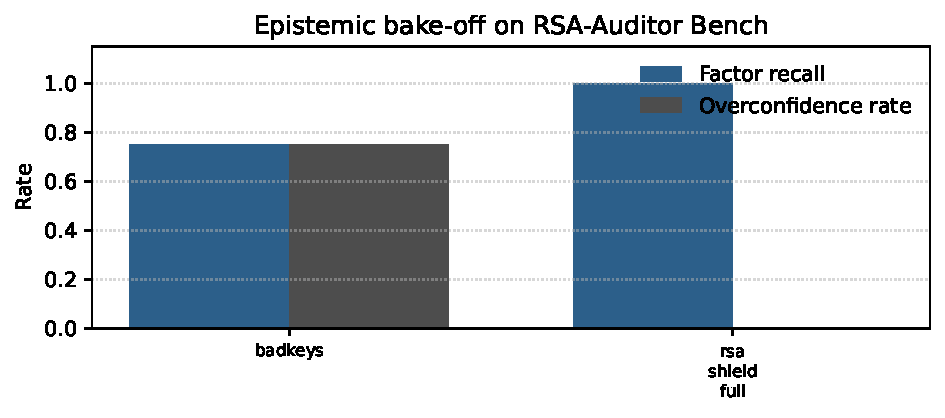
\includegraphics[width=\columnwidth,height=2.1in,keepaspectratio]{figures/fig_bakeoff.pdf}
\caption{Factor recall vs.\ overconfidence on RSA-Auditor Bench (\texttt{bakeoff.json}).}
\label{fig:bakeoff}
\end{figure}

\begin{table}[t]
\caption{Epistemic bake-off aggregates (\texttt{bakeoff.json}).}
\label{tab:bakeoff}
\centering
\resizebox{\columnwidth}{!}{%
\begin{tabular}{lcccc}
\toprule
\textbf{Tool} & \textbf{Recall} & \textbf{FP rate} & \textbf{Overconf.} & \textbf{Notes} \\
\midrule
RSA-SHIELD full & 1.00 & 0.00 & 0.00 & TP${=}4$, FN${=}0$; never \texttt{SECURE} \\
\texttt{badkeys} & 0.75 & 0.00 & 0.75 & TP${=}3$, FN${=}1$; empty${=}$OK-like \\
\texttt{RsaCtfTool} & --- & --- & --- & Not installed (availability-only) \\
\bottomrule
\end{tabular}%
}
\end{table}

Table~\ref{tab:bakeoff}: RSA-SHIELD recovers all four planted factor classes with overconfidence $0/3$. \texttt{badkeys} recovers three (misses the smoothish/\texttt{weak-ecm} class under default checks) and yields overconfidence $3/4$ because empty findings on non-hits read as OK. Per-fixture detail (from \texttt{bakeoff.json} rows): \texttt{badkeys} flagged \texttt{small-factor} (\texttt{smallfactors}), \texttt{fermat-close} (\texttt{fermat}), and \texttt{wiener-small-d} (\texttt{smalld}); returned empty OK-like results on \texttt{weak-ecm}, \texttt{normal-demo}, and \texttt{legacy-1024}. RSA-SHIELD labeled the last two \texttt{SUSPICIOUS} (size/ROCA heuristics) rather than pass. This is complementarity, not a claim that \texttt{badkeys} is ``wrong'' for fingerprinting---it shows why never-\texttt{SECURE} tiers matter for defensive audits.

Motivating deployments for the auditor---shared-prime collisions after low-entropy embedded provisioning~\cite{heninger2012mining,hastings2016weak} and ROCA-class smartcard inventories~\cite{nemec2017return}---motivate inventory GCD and fingerprint tiers, but remain scenarios rather than a new field measurement campaign in this paper.

\subsection{Fixture Suite}
Table~\ref{tab:suite}: $7/7$ hint matches; four factor methods; two \texttt{SUSPICIOUS}; one \texttt{INVALID\_KEY}; zero \texttt{SECURE}.

\begin{table}[t]
\caption{Controlled fixture suite (ECM timeout $2500$\,ms; \texttt{suite.json}).}
\label{tab:suite}
\centering
\resizebox{\columnwidth}{!}{%
\begin{tabular}{llcc}
\toprule
\textbf{Fixture} & \textbf{Observed state} & \textbf{Method} & \textbf{ms} \\
\midrule
weak-ecm & \texttt{FACTOR\_FOUND} & ECM & 36.51 \\
small-factor & \texttt{FACTOR\_FOUND} & TINY\_FACTOR & 0.16 \\
fermat-close & \texttt{FACTOR\_FOUND} & FERMAT & 0.13 \\
wiener-small-d & \texttt{FACTOR\_FOUND} & WIENER & 9.48 \\
normal-demo & \texttt{SUSPICIOUS} & --- & 2508.7 \\
legacy-1024 & \texttt{SUSPICIOUS} & --- & 8050.87 \\
invalid-pem & \texttt{INVALID\_KEY} & --- & 0 \\
\bottomrule
\end{tabular}%
}
\end{table}

\subsection{Ablation and Configuration Comparison}
Fig.~\ref{fig:ablation} / Table~\ref{tab:ablation}: complementary probes. Fig.~\ref{fig:config} / Table~\ref{tab:config}: full pipeline precision/recall $1.0$ (TP${=}4$, FP${=}0$, FN${=}0$), avg $861.14$\,ms.

\begin{figure}[t]
\centering
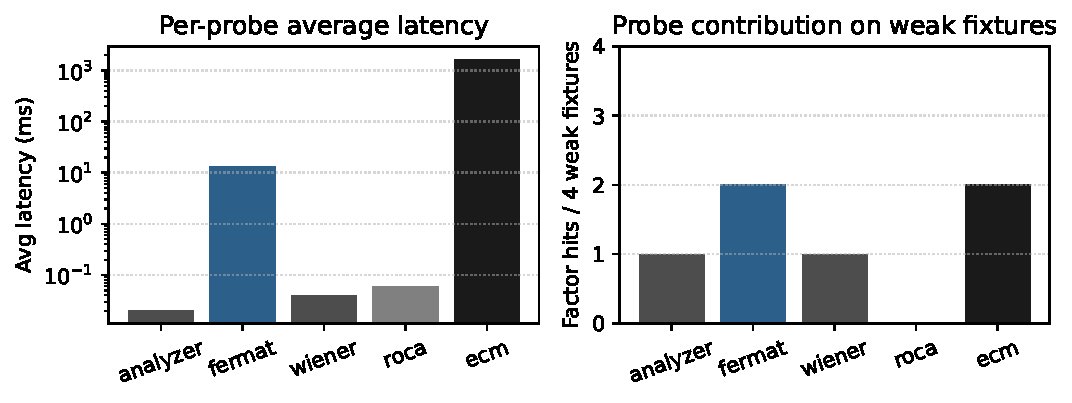
\includegraphics[width=\columnwidth,height=2.1in,keepaspectratio]{figures/fig_ablation_latency.pdf}
\caption{Ablation on weak fixtures (\texttt{ablation.json}).}
\label{fig:ablation}
\end{figure}

\begin{table}[t]
\caption{Ablation summary on four weak fixtures (\texttt{ablation.json}).}
\label{tab:ablation}
\centering
\resizebox{\columnwidth}{!}{%
\begin{tabular}{lccc}
\toprule
\textbf{Probe} & \textbf{Hits / 4} & \textbf{Hit rate} & \textbf{Avg ms} \\
\midrule
analyzer & 1 & 0.25 & 0.02 \\
fermat & 2 & 0.50 & 13.29 \\
wiener & 1 & 0.25 & 0.04 \\
roca & 0 & 0.00 & 0.06 \\
ecm & 2 & 0.50 & 1682.63 \\
\bottomrule
\end{tabular}%
}
\end{table}

\begin{figure}[t]
\centering
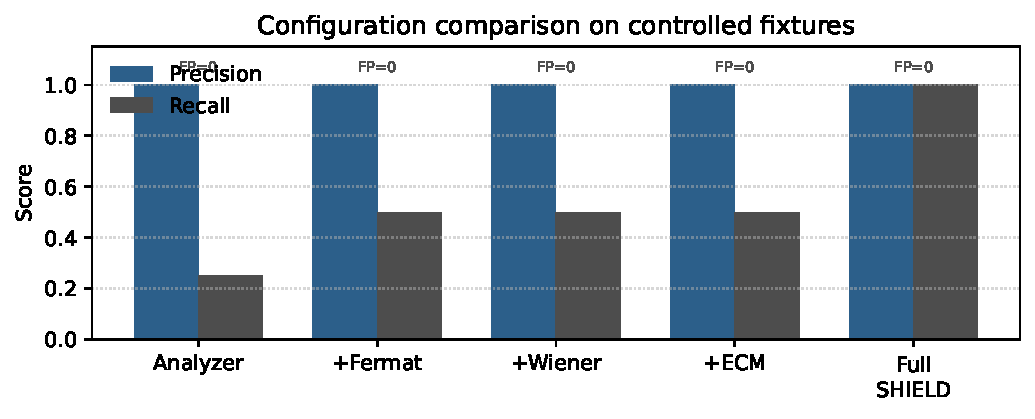
\includegraphics[width=\columnwidth,height=2.1in,keepaspectratio]{figures/fig_config_recall.pdf}
\caption{Configuration precision/recall (\texttt{comparison.json}).}
\label{fig:config}
\end{figure}

\begin{table}[t]
\caption{Configuration aggregates (\texttt{comparison.json}).}
\label{tab:config}
\centering
\resizebox{\columnwidth}{!}{%
\begin{tabular}{lcccccc}
\toprule
\textbf{Config} & \textbf{TP} & \textbf{FP} & \textbf{FN} & \textbf{Prec.} & \textbf{Rec.} & \textbf{Avg ms} \\
\midrule
Analyzer only & 1 & 0 & 3 & 1.00 & 0.25 & 0.03 \\
Analyzer+Fermat & 2 & 0 & 2 & 1.00 & 0.50 & 13.96 \\
Analyzer+Wiener & 2 & 0 & 2 & 1.00 & 0.50 & 0.07 \\
Analyzer+ECM & 2 & 0 & 2 & 1.00 & 0.50 & 1676.16 \\
Full SHIELD & 4 & 0 & 0 & 1.00 & 1.00 & 861.14 \\
\bottomrule
\end{tabular}%
}
\end{table}

\subsection{Batch-GCD Scaling}
Synthetic $\approx 512$-bit moduli (two $256$-bit primes), one planted shared prime. Parity verified at every size. At $N{=}1000$, pairwise $1246.17$\,ms vs.\ tree $645.79$\,ms ($1.93\times$). At $N{=}20$, tree overhead can lose ($0.82\times$)---reported honestly.

\begin{figure}[t]
\centering
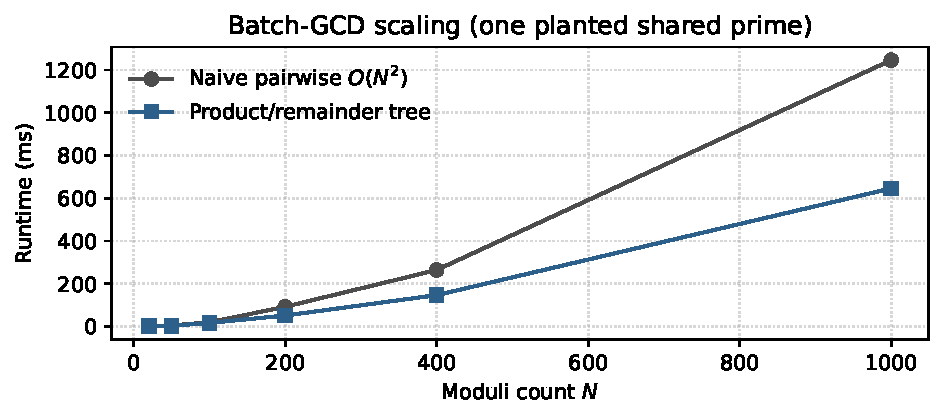
\includegraphics[width=\columnwidth,height=2.1in,keepaspectratio]{figures/fig_batch_gcd_scale.pdf}
\caption{Batch-GCD scaling through $N{=}1000$ (\texttt{batch\_gcd\_benchmark.json}).}
\label{fig:batch}
\end{figure}

\begin{table}[t]
\caption{Batch-GCD scaling (measured; one shared prime planted).}
\label{tab:batch}
\centering
\resizebox{\columnwidth}{!}{%
\begin{tabular}{cccccc}
\toprule
$N$ & Pairs & Naive (ms) & Tree (ms) & Speedup & Parity \\
\midrule
20 & 190 & 0.57 & 0.70 & $0.82\times$ & Yes \\
50 & 1{,}225 & 4.19 & 2.81 & $1.49\times$ & Yes \\
100 & 4{,}950 & 19.01 & 16.28 & $1.17\times$ & Yes \\
200 & 19{,}900 & 91.85 & 50.79 & $1.81\times$ & Yes \\
400 & 79{,}800 & 263.97 & 146.34 & $1.80\times$ & Yes \\
1000 & 499{,}500 & 1246.17 & 645.79 & $1.93\times$ & Yes \\
\bottomrule
\end{tabular}%
}
\end{table}

\subsection{Mini Synthetic Corpus}
Corpus $n{=}40$: shared-prime pair ($2$), four single-key weak classes ($1$ each), $34$ normals (Fig.~\ref{fig:corpus}, Table~\ref{tab:corpus_counts}). Single-key factors $4$; batch-GCD hits $1$ in $0.31$\,ms over $780$ pair-equivalents; \texttt{SECURE}${=}0$. All $40$ moduli are under $1024$ bits. Shared-prime keys contribute zero single-key factor finds until inventory GCD runs.

\begin{figure}[t]
\centering
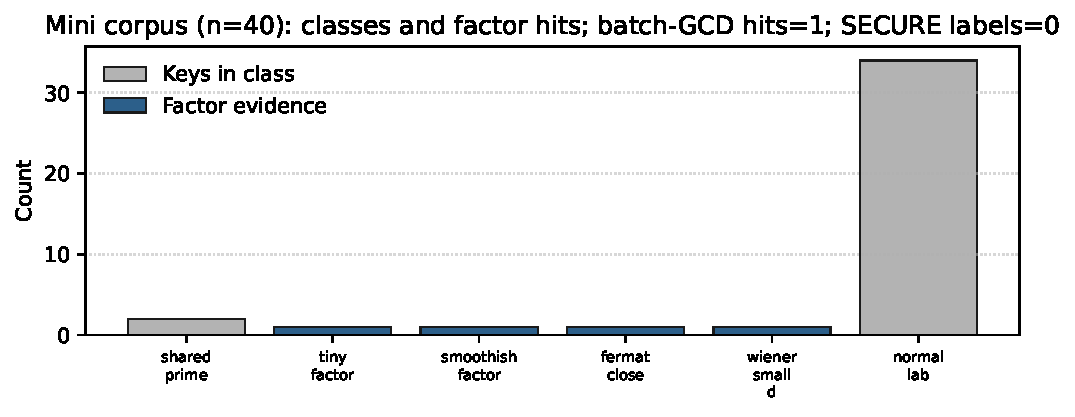
\includegraphics[width=\columnwidth,height=2.1in,keepaspectratio]{figures/fig_corpus_states.pdf}
\caption{Mini corpus classes vs.\ single-key factor evidence.}
\label{fig:corpus}
\end{figure}

\begin{table}[t]
\caption{Mini corpus composition (\texttt{corpus.json}).}
\label{tab:corpus_counts}
\centering
\resizebox{\columnwidth}{!}{%
\begin{tabular}{lcc}
\toprule
\textbf{Class} & \textbf{Count} & \textbf{Single-key factors} \\
\midrule
shared\_prime & 2 & 0 \\
tiny\_factor & 1 & 1 \\
smoothish\_factor & 1 & 1 \\
fermat\_close & 1 & 1 \\
wiener\_small\_d & 1 & 1 \\
normal\_lab & 34 & 0 \\
\midrule
\textbf{Total} & 40 & 4 factors; 1 GCD hit; 0 \texttt{SECURE} \\
\bottomrule
\end{tabular}%
}
\end{table}

\subsection{Public CT Sample Measurement}
\label{sec:ct}
To move beyond purely synthetic fixtures, we sampled \textbf{three} contemporary public CT logs (Google Argon2026h2, Google Xenon2026h2, Cloudflare Nimbus2026) via RFC~6962 \texttt{get-entries} and extracted unique RSA moduli (script \texttt{paper/scripts/ct\_measurement.py}). The multi-log tip crawl examined $19504$ leaf entries and produced \textbf{$12010$ unique moduli} in $1586.86$\,s (per-log unique adds: $4011$+$4013$+$3986$; bit lengths: $11654\times 2048$, $336\times 4096$, $20\times 3072$).

Because a single product tree over $>10^{4}$ $2048$-bit moduli is memory-infeasible in our lab setting, we ran \textbf{chunked} batch GCD (chunk size $250$, two passes including a shuffled pass). Result: \textbf{$0$ shared-factor hits} in $81172.63$\,ms---consistent with prior observations that modern CT corpora show far fewer shared primes than historical IoT/TLS scans~\cite{heninger2012mining,hastings2016weak}. Chunking may miss some cross-window shares; we state this limitation explicitly.

\begin{figure}[t]
\centering
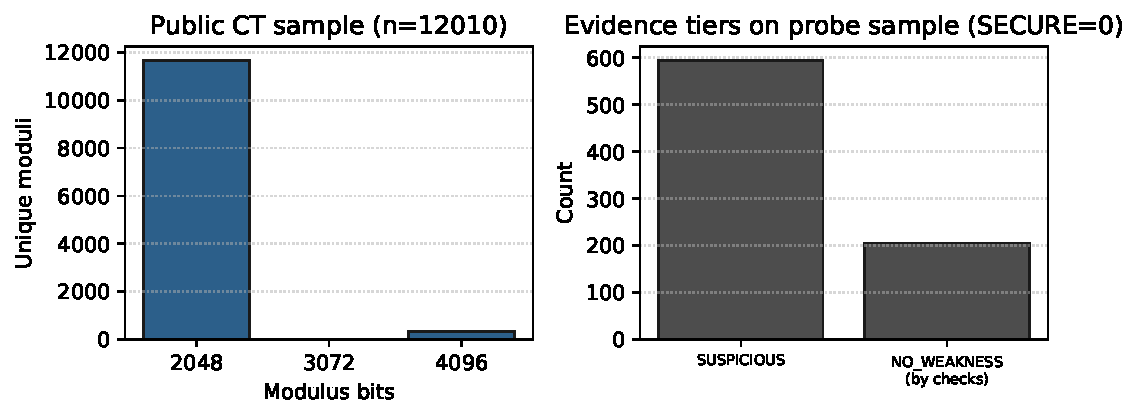
\includegraphics[width=\columnwidth,height=2.2in,keepaspectratio]{figures/fig_ct_measurement.pdf}
\caption{Multi-log public CT sample: bit-length histogram and evidence-tier counts on an $800$-key probe sample (\texttt{ct\_measurement.json}).}
\label{fig:ct}
\end{figure}

On an $800$-key evidence-tier probe sample (analyzer + \emph{legacy} educational ROCA; ECM omitted at CT scale under lab budgets), RSA-SHIELD emitted \textbf{$0$ \texttt{SECURE}} labels: $594$ \texttt{SUSPICIOUS} and $206$ \texttt{NO\_WEAKNESS\_DETECTED\_BY\_CONFIGURED\_CHECKS}. All $594$ suspicious flags came from the legacy ROCA heuristic ($74.25\%$ of the sample)---motivating the calibration study below. Tiny-factor hits were $0$; no modulus under $2048$ bits appeared in this tip sample.

\subsection{ROCA Fingerprint Parity and Calibration}
\label{sec:roca}
We compared the educational ROCA heuristic to \texttt{badkeys}' \texttt{roca} finding on Bench fixtures and public CT tip samples. Under the \emph{legacy} educational profile on the calibration set ($n{=}500$), positives were $375/500$ ($75\%$) while \texttt{badkeys} reported \textbf{$0$} ROCA hits (agreement only $25\%$). Sweeping $(\texttt{ratio\_threshold},\texttt{min\_gcd})$ against \texttt{badkeys} selected a \emph{calibrated} profile ($\texttt{ratio\_threshold}{=}0.99$, $\texttt{min\_gcd}{=}2$): false positives fell to $1/500$ ($0.2\%$), agreement rose to $99.8\%$, and FP-rate reduction was $0.9973$ (\texttt{roca\_calibration.json}). An independent parity re-check ($n{=}400$) confirmed calibrated agreement $100\%$ vs.\ legacy $25.25\%$ (\texttt{roca\_parity.json}). Bench agreement under calibrated defaults is $7/7$. The shipped detector uses the calibrated profile by default; positives remain \texttt{SUSPICIOUS} only---fingerprint $\neq$ Coppersmith factorization (Fig.~\ref{fig:roca}).

\begin{figure}[t]
\centering
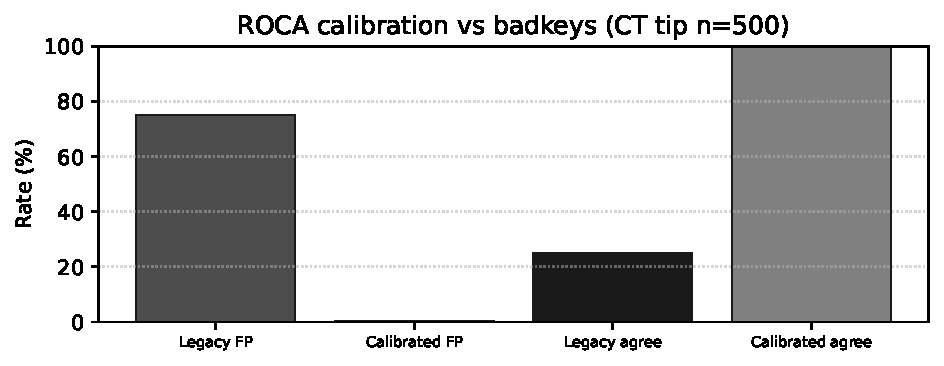
\includegraphics[width=\columnwidth,height=2.15in,keepaspectratio]{figures/fig_roca_parity.pdf}
\caption{Legacy vs.\ calibrated educational ROCA vs.\ \texttt{badkeys} on a CT tip sample (\texttt{roca\_calibration.json}).}
\label{fig:roca}
\end{figure}

\subsection{Adaptive Probe Scheduler}
\label{sec:adaptive}
Fixed budgets waste work on $2048$-bit CT-like keys (near-twin Fermat rarely helps). Our adaptive planner shrinks/skips Fermat and trims Pollard/ECM budgets for large bit-lengths while keeping aggressive budgets for small/legacy keys and large-$e$ Wiener cases. On Bench fixtures, fixed mean wall time was $1473.92$\,ms vs.\ adaptive $975.75$\,ms ($1.511\times$), with factor recall unchanged at $1.0$ (TP${=}5$/FN${=}0$ including the Pollard fixture) and zero \texttt{SECURE} labels (Fig.~\ref{fig:adaptive}).

\begin{figure}[t]
\centering
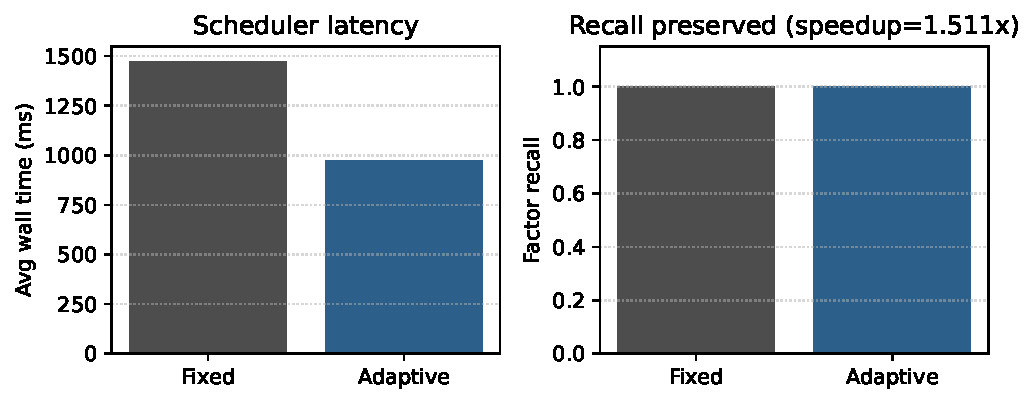
\includegraphics[width=\columnwidth,height=2.1in,keepaspectratio]{figures/fig_adaptive.pdf}
\caption{Fixed vs.\ adaptive probe budgets on RSA-Auditor Bench (\texttt{adaptive\_ablation.json}).}
\label{fig:adaptive}
\end{figure}

\subsection{Discussion}
Bake-off overconfidence, ROCA parity disagreement, and adaptive latency-with-preserved-recall are the headline systems results. Classical probes remain the engine; batch microbenchmarks are supporting. Precision $1.0$ on Bench is not a production CVE false-positive rate.

\section{Implementation and Reproducibility}
FastAPI + React/Vite; evaluation endpoints regenerate Tables~\ref{tab:bakeoff}--\ref{tab:batch}. Budgets: Fermat $25{,}000$ steps, ECM $2500$\,ms baseline; probe order analyzer$\rightarrow$Fermat$\rightarrow$Wiener$\rightarrow$ROCA$\rightarrow$Pollard~$p{-}1$$\rightarrow$ECM with short-circuit on first factor. Workflow: \texttt{export\_benchmark.py}, \texttt{dump\_eval\_data.py} (includes bake-off), \texttt{generate\_figures.py}, \texttt{audit\_paper\_claims.py}. Large Wiener exponents are stored as decimal strings to avoid $64$-bit SQLite overflow. Responsible use: authorized public keys only; never paraphrase inconclusive as certification. Re-running on another machine may change wall-clock milliseconds; structural counts (hint matches, TP/FP/FN, bake-off overconfidence numerators, batch parity) are the intended cross-machine invariants.

\section{Related Work}
\paragraph{Measurement and batch GCD.}
Heninger et al.~\cite{heninger2012mining}, Hastings et al.~\cite{hastings2016weak}, and Lenstra et al.~\cite{lenstra2012ron} established Internet-scale weak-key measurement via batch GCD; Bernstein trees~\cite{bernstein2004find} supply the algorithmic substrate. RSA-SHIELD reuses that substrate inside a defensive auditor and does not repeat a global Certificate Transparency crawl.

\paragraph{Classical attacks.}
Wiener~\cite{wiener1990cryptanalysis}, Boneh--Durfee~\cite{boneh2000cryptanalysis}, Coppersmith~\cite{coppersmith1997small}, Nemec et al.~\cite{nemec2017return}, and Lenstra ECM~\cite{lenstra1987factoring} are the attacks we bound and orchestrate. Our ROCA path is an educational fingerprint, not a lattice factorization pipeline.

\paragraph{Tooling niches.}
\texttt{badkeys}~\cite{bock2022badkeys} and \texttt{RsaCtfTool}~\cite{rsactftool} occupy fingerprint vs.\ CTF niches. Prior work rarely publishes a small labeled auditor bench with an explicit overconfidence metric that treats empty/pass-like outputs as a first-class failure mode. That evaluation artifact---not a new attack---is our systems contribution.

\section{Limitations and Threats to Validity}
Bench v1.0 recall $1.0$ is relative to planted weak classes only. The CT study is a multi-log \emph{tip sample} ($12010$ moduli across three logs), not a billion-certificate census; chunked batch GCD can miss cross-window shares; ECM was not run on the CT sample. ROCA parity uses \texttt{badkeys} as a fingerprint reference, not ground-truth Infineon compromise. Adaptive speedups are Bench-specific. Batch milliseconds are machine-specific. Future work: larger crawls, crocs-roca cross-checks, optional NIST FIPS~203/204~\cite{nist2024fips203,nist2024fips204} hints---without relaxing never-\texttt{SECURE}.

\section{Ethical Considerations}
RSA-SHIELD is a defensive auditor for authorized public keys. It rejects private material at ingest and never maps timeouts to a security certification. Operators must not scan inventories without authorization. Educational ROCA fingerprint hits require independent confirmation before remediation. Synthetic planted collisions are for pedagogy and regression testing; they are not a substitute for consent-based measurement studies of production PKI.

\section{Artifact Availability}
Artifacts include Bench v1.0, frozen JSON (\texttt{bakeoff.json}, \texttt{ct\_measurement.json}, \texttt{roca\_parity.json}, \texttt{roca\_calibration.json}, \texttt{adaptive\_ablation.json}), and scripts \texttt{run\_roca\_parity.py}, \texttt{run\_roca\_calibration.py}, \texttt{run\_adaptive\_ablation.py}, \texttt{ct\_measurement.py}. Optional: \texttt{pip install badkeys}. CT uses public RFC~6962 APIs only.

\section{Conclusion}
RSA-SHIELD couples never-\texttt{SECURE} auditing with Bench/bake-off, CT measurement, calibrated ROCA parity, and adaptive scheduling. Headline measured results: overconfidence $0.0$ vs.\ \texttt{badkeys} $0.75$; ROCA FP $75\%\!\rightarrow\!0.2\%$ after calibration ($n{=}500$); adaptive $1.511\times$ faster at recall $1.0$. Classical probes remain the engine; the citable contribution is evidence-correct systems evaluation.

\bibliographystyle{IEEEtran}
\bibliography{references}

\end{document}
